% 6.5 下午2点预答辩
\documentclass[10pt]{beamer}

\usepackage{beamerthemesplit}
\usepackage{times}
\usefonttheme{structurebold}
\usepackage[english]{babel}
\usepackage{pgf,pgfarrows,pgfnodes,pgfautomata,pgfheaps}
\usepackage{amsmath,amssymb}
\usepackage[latin1]{inputenc}
\usepackage{multimedia}
\setcounter{equation}{0}
\numberwithin{equation}{section}
\setbeamercovered{dynamic}

\newcommand{\Lang}[1]{\operatorname{\text{\textsc{#1}}}}
\newcommand{\Class}[1]{\operatorname{\mathchoice
  {\text{\sf \small #1}}
  {\text{\sf \small #1}}
  {\text{\sf #1}}
  {\text{\sf #1}}}}

\newcommand{\NumSAT}      {\text{\small\#SAT}}
\newcommand{\NumA}        {\#_{\!A}}
\newcommand{\barA}        {\,\bar{\!A}}
\newcommand{\Nat}{\mathbb{N}}
\newcommand{\Set}[1]{\{#1\}}

\usepackage[latin1]{inputenc}
\usepackage{beamerthemesplit}
\usepackage{pgf,pgfarrows,pgfnodes,pgfautomata,pgfheaps,pgfshade}
\usepackage{graphicx}
\usepackage{subfloat}
\usepackage{chemarrow}
\usepackage{epsfig, subfigure}
\usepackage{latexsym,amssymb,lastpage}
\usepackage{graphicx,amsfonts}
\usepackage{times,mathptmx,bm,amsmath}
\usepackage{dcolumn}
\newcommand{\me}{\mathrm{e}}
\newcommand{\mi}{\mathrm{i}}
\newcommand{\md}{\mathrm{d}}

\usefonttheme{professionalfonts}
\usefonttheme{serif}

\def\mathfamilydefault{\rmdefault}

\usepackage{fontspec}
\setmainfont{Lucida Bright}

\newcommand{\nq}{\\[5pt]}
\newcommand{\nw}{\\[10pt]}

\setbeamercovered{transparent}
% \usetheme{m}
\usetheme{Madrid}
% \usecolortheme{dolphin}

\pgfdeclareimage[height=.8cm]{logo}{fd1.eps}

\title[Statistics of Solutions to Test Models for SPEKF]{\huge Statistics of Solutions to Test Models for SPEKF}
\author[Chuan Lu]{\Large{Chuan Lu}}
\institute[ICS]{\large{Information and Computing Science}\linebreak \linebreak
\pgfuseimage{logo}
}
\date{June 2017}

\AtBeginSection[]{\frame{\frametitle{Outline}\tableofcontents[current]}}

\begin{document}

\frame{\titlepage}
\newcommand{\E}{\text{E}}
\newcommand{\Cov}{\text{Cov}}
\newcommand{\Var}{\text{Var}}
\renewcommand{\v}{\mathbf{v}}
\newcommand{\s}{\mathbf{s}}
\newcommand{\ii}{\mathrm{i}}
\newcommand{\dotW}{\dot{W}}
% \frame{\tableofcontents[all]}

\section{Introduction}

\subsection{Stochastic Parameterization Extended Kalman Filter (SPEKF)}

\begin{frame}\frametitle{Introduction}
Signals from nature can be modeled by Langevin equation:
\begin{block}{Langevin Equation}
\[
\frac{\mathrm{d}u(t)}{\mathrm{d}t} = -\gamma(t)u(t) + \ii\omega u(t)+\sigma \dotW(t)+f(t),
\]
where $\dotW(t)$ is a Brownian motion, and $f(t)$ is the external force. 
\end{block}

A major difficulty in accurate filtering of noisy signals with many degrees of freedom is model error; signal from nature is processed through incomplete physical models, as well as parameterized to inadequate numerical resolution.\\[10pt]

B. Gershgorin, \textit{et, al} proposed the Stochastic Parameterization Extended Kalman Filter (SPEKF) to cope with model errors.
\end{frame}

\frame{\frametitle{Introduction}
\begin{block}{Test Model}
\[
\left\{
\begin{aligned}
& \frac{du(t)}{dt} = (-\gamma(t)+\ii\omega)u(t)+b(t)+f(t)+\sigma W(t), \nq
& \frac{db(t)}{dt} = (-\gamma_b+\ii\omega_b)(b(t)-\hat{b})+\sigma_b W_b(t), \nq
& \frac{d\gamma(t)}{dt} = -d_\gamma(\gamma(t)-\hat{\gamma})+\sigma_\gamma W_\gamma(t)
\end{aligned}
\right.
\]
\end{block}
The initial values are complex random variables, with their first-order and second-order statistics known. }

\frame{\frametitle{Introduction}
\begin{block}{Solution}
With knowledge of ODEs, solution of the SDE set is
\[
\left\{
\begin{aligned}
& b(t) = \hat{b}+(b_0-\hat{b})e^{\lambda_b(t-t_0)}+\sigma_b\int_{t_0}^t e^{\lambda_b(t-s)}dW_b(s) \nq
& \gamma(t) = \hat{\gamma}+(\gamma_0-\hat{\gamma})e^{-d_{\gamma}(t-t_0)}+\sigma_{\gamma}\int_{t_0}^t e^{-d_{\gamma}(t-s)}dW_{\gamma}(s) \nq
& u(t) = e^{-J(t_0, t)+\hat{\lambda}(t-t_0)}u_0 + \int_{t_0}^t (b(s)+f(s))e^{-J(s, t)+\hat{\lambda}(s-t_0)}ds \nq
&\quad\quad + \sigma\int_{t_0}^{t}e^{-J(s, t)+\hat{\lambda}(s-t_0)}dW(s)
\end{aligned}
\right.
\]
\end{block}
with $\lambda_b = -\gamma_b+\ii\omega_b$, ~$\hat{\lambda} = -\hat{\gamma}+\ii\omega$, ~$J(s, t) = \int_s^t (\gamma(s')-\hat{\gamma})ds'$.
}

\subsection{It\^o Integration}
\frame{\frametitle{Introduction}
\begin{block}{It\^o Isometry}
$\forall f\in\mathcal{V}(S, T)$, $B_t$ is a standard Brownian motion,
$$\E\left[\left(\int_S^T f(t, \omega)dB_t\right)^2\right] = \E\left[\int_S^T f^2(t, \omega)dt\right].$$
\end{block}	


\begin{block}{Linear property of It\^o integration}
$$
\begin{aligned}
& (1)\quad \int_S^T fdB_t = \int_S^U fdB_t + \int_U^T fdB_t, ~\text{a.e.}\nq
& (2)\quad \int_S^T (cf+g)dB_t = c\int_S^T fdB_t + \int_S^T gdB_t, ~\text{a.e.}\nq
& (3)\quad \E\left[\int_S^T fdB_t\right] = 0.
\end{aligned}
$$
\end{block}
}

\section{Statistics of $b(t)$ and $\gamma(t)$}
\subsection{Mean}
\frame{\frametitle{Mean of $b(t)$, $\gamma(t)$}
\quad With property of It\^o integration (3), the last term in $\E[b(t)]$ is $0$. \\
\quad Thus we find
\begin{block}{}
$$
\begin{aligned}
&\E[b(t)] = \hat{b} + (\E[b_0] - \hat{b})e^{\lambda_b(t-t_0)} \nq
&\E[\gamma(t)] = \hat{\gamma} + (\E[\gamma_0] - \hat{\gamma})e^{-d_{\gamma}(t-t_0)}
\end{aligned}
$$
\end{block}
}

\subsection{Variance}
\frame{\frametitle{Variance of $b(t)$, $\gamma(t)$}
\quad According to definition, 
\[
\begin{aligned}
\text{Var}&(b(t)) = \E\left[(b(t)-\E[b(t)])(b(t)-\E[b(t)])^*\right] \nq
&= e^{-2\gamma_b(t-t_0)}\Var(b_0) + \E\left[\sigma_b^2\int_{t_0}^t e^{\lambda_b(t-s)}dW_b(s)\left(\int_{t_0}^t e^{\lambda_b(t-s)}dW_b(s)\right)^*\right] \nq
&= e^{-2\gamma_b(t-t_0)}\Var(b_0) + \sigma_b^2\E\left[\int_{t_0}^t e^{-2\gamma_b(t-s)}ds\right]
\end{aligned}
\]
\quad The last step takes use of It\^o isometry. Compute the integration in last term, we have
\begin{block}{}
\[
\begin{aligned}
&\Var(b(t)) = e^{-2\gamma_b(t-t_0)}\Var(b_0) + \frac{\sigma_b^2}{2\gamma_b}(1-e^{-2\gamma_b(t-t_0)}) \nq
&\Var(\gamma(t)) = e^{-2d_\gamma(t-t_0)}\Var(\gamma_0) + \frac{\sigma_\gamma^2}{2d_\gamma}(1-e^{-2d_\gamma(t-t_0)})
\end{aligned}
\]
\end{block}
}

\subsection{Covariance}
\frame{\frametitle{Covariance of $b(t)$, $\gamma(t)$}
According to definition,
\[
\begin{aligned}
\Cov&(b(t), b(t)^*) = \E\left[(b(t) - \E[b(t)])(b(t)^* - \E[b(t)^*])\right] \nw
&= \E\left[(b_0 - \E[b_0])(b_0^* - \E[b_0^*])e^{2\lambda_b (t-t_0)}\right] + \sigma_b\E\left[(b_0 - \E[b_0])\int_{t_0}^{t}e^{\lambda_b(t-s)}dW_b(s)\right]\nq
&+ \sigma_b\E\left[(b_0^*-\E[b_0^*])e^{\lambda_b(t-t_0)}\int_{t_0}^{t}e^{\lambda_b(t-s)}dW_b(s)\right] + \sigma_b^2\E\left[(\int_{t_0}^{t}e^{\lambda_b(t-s)}dW_b(s))^2\right]
\end{aligned}
\]
\quad With property of It\^o integration (3), the second and third term are both 0; with It\^o isometry we know the last term is also 0. Accordingly,
\begin{block}{}
\[
\begin{aligned}
&\Cov(b(t), b(t)^*) = \E[(b_0-\E[b_0])(b_0^*-\E[b_0^*])]e^{2\lambda_b(t-t_0)} = \Cov(b_0, b_0^*)e^{2\lambda_b(t-t_0)} \nq
&\Cov(b(t), \gamma(t)) = \E[(b(t) - \E[b(t)])(\gamma(t)-\E[\gamma(t)])]= \Cov(b_0, \gamma_0)e^{(\lambda_b-d_\gamma)(t-t_0)}
\end{aligned}
\]
\end{block}
}

\section{Statistics of $u(t)$}
\subsection{Mean}
\frame{\frametitle{Mean of $u(t)$}
\quad Using the same properties, it is easy to find
\[
\begin{aligned}
\E[u(t)] &= e^{\hat{\lambda}(t-t_0)}\E\left[e^{-J_0(t_0, t)}u_0\right] + \int_{t_0}^t e^{\hat{\lambda}(t-s)}\E\left[b(s)e^{-J(s, t)}\right]ds  \nq
&+ \sigma\int_{t_0}^{t} e^{\hat{\lambda}(t-s)}f(s)\E\left[e^{-J(s, t)}\right]ds.
\end{aligned}
\]
\quad We find it necessary to compute expectations of terms like
\[
\E[ze^{bx}],
\]
where $z$ is a complex-valued Gaussian random variable and x is a real-valued Gaussian variable. We propose two lemmas here.
}

\frame{\frametitle{Mean of $u(t)$}
\begin{lemma}[1]\label{lemma 1}
$$\E\left[ze^{\ii bx}\right] = (\E[z]+\ii b\Cov(z, x))e^{\ii b\E[x]-\frac{1}{2}b^2\Var(x)},$$
with $z$ being a complex-valued Gaussian, and $x$ a real-valued Gaussian.
\end{lemma}

\begin{Corollary}[1] \label{corollary 1}
Under the condition of Lemma \ref{lemma 1},
$$\E\left[ze^{bx}\right] = (\E[z]+b\Cov(z, x))e^{b\E[x]+\frac{1}{2}b^2\Var(x)}.$$
\end{Corollary}
Proof of lemma \ref{lemma 1} takes advantage of characteristic function of multivariable Gaussian distribution.
}

\frame{\frametitle{Proof}

\quad Let $z = y+\ii w, ~y, w \in \mathbb{R}.$ Denote $\v = (x, y, w)^\top$, then $\v$ satisfies the multivariable Gaussian distribution, with its characteristic function
\[
\phi_\v(\s) = \exp(\ii\s^\top\E[\v]-\frac{1}{2}\s^\top\Sigma\s).
\]
\quad Let $g(\v)$ being the PDF of $\v$, then one knows from that char. func. being Fourier transform of PDF,
\[
\phi_\v(\s) = \frac{1}{(2\pi)^3}\int e^{\ii\s^\top\v}g(\v)d\v.`'
\]
\quad According to the differential property of Fourier transform (Proposition 2.10), 
\[
\frac{\partial \phi_\mathbf{v}(\mathbf{s})}{\partial s_2} = \frac{1}{(2\pi)^3}\int \ii y_0e^{\ii\mathbf{s}^\top\mathbf{v}}g(\mathbf{v})d\mathbf{v} = \ii\E\left[y_0e^{\ii\mathbf{s}^\top\mathbf{v}}\right].
\]
\quad Let $\v = (b, 0, 0)^\top$, 
\[
\left.\E[y_0e^{\ii bx_0}] = -\ii\frac{\partial \phi_\mathbf{v}(s)}{\partial s_2}\right|_{\mathbf{s} = (b, 0, 0)^\top}, ~
\left.\E[w_0e^{\ii bx_0}] = -\ii\frac{\partial \phi_\mathbf{v}(s)}{\partial s_3}\right|_{\mathbf{s} = (b, 0, 0)^\top}
\]
}

\frame{\frametitle{Proof}
\quad From PDF of multivariable Gaussian distribution, one knows
\[
\begin{aligned}
&\frac{\partial \phi_\mathbf{v}(\mathbf{s})}{\partial s_2} = (\ii\E[y_0]-\Var(y_0)s_2-\Cov(x_0, y_0)s_1-\Cov(y_0, w_0)s_3)\phi_{\mathbf{v}}(s) \nq
&\frac{\partial \phi_\mathbf{v}(\mathbf{s})}{\partial s_3} = (\ii\E[w_0]-\Var(w_0)s_3-\Cov(x_0, w_0)s_1-\Cov(y_0, w_0)s_2)\phi_{\mathbf{v}}(s)
\end{aligned}
\]
\quad Compute the partial derivatives at $\s = (b, 0, 0)^\top$,
\[
\begin{aligned}
&\E\left[y_0e^{\ii bx_0}\right] = (\E[y_0]+\ii\Cov(x_0, y_0)b)\exp(\ii b\E[x_0] - \frac{1}{2}\Var(x_0)b^2) \nq
&\E\left[w_0e^{\ii bx_0}\right] = (\E[w_0]+\ii\Cov(x_0, w_0)b)\exp(\ii b\E[x_0] - \frac{1}{2}\Var(x_0)b^2)
\end{aligned}
\]
\quad Then $$\E\left[ze^{\ii bx}\right] = (\E[z]+\ii b\Cov(z, x))e^{\ii b\E[x]-\frac{1}{2}b^2\Var(x)}.$$ \qed
}

\frame{\frametitle{Mean of $u(t)$}
\begin{lemma}[2] \label{lemma 2}
\[
\begin{aligned}
\E\left[zwe^{bx}\right] &= \left[\E[z]\E[w]+\Cov(z, w^*)+b(\E[z]\Cov(w, x))+\E[w]\Cov(z, x)+ \right. \nq
& \left.b^2\Cov(z, x)\Cov(w, x)\right]e^{b\E[x]+\frac{b^2}{2}\Var(x)}. \\
\end{aligned}
\]
with $z, w$ being complex-valued Gaussian, and $x$ real-valued Gaussian.
\end{lemma}
The proof of this lemma is the same as Lemma \ref{lemma 1}.
}

\frame{\frametitle{Mean of $u(t)$}
\quad We now make use of Lemma \ref{lemma 1} to obtain mean of $u(t)$.
\begin{block}{}
\[
\begin{aligned}
&\E[u(t)] = e^{\hat{\lambda}(t-t_0)}(\E[u_0]-\Cov(u_0, J(t_0, t)))e^{-\E[J(t_0, t)]+\frac{1}{2}\Var(J(t_0, t))} \nw
&\quad\quad+ \int_{t_0}^t e^{\hat{\lambda}(t-s)}(\hat{b}+e^{\lambda_b(s-t_0)}(\E[b_0]-\hat{b}-\Cov(b_0, J(s, t))))e^{-\E[J(s, t)]+\frac{1}{2}\Var(J(s, t))}ds \nq
&\quad\quad+ \int_{t_0}^t e^{\hat{\lambda}(t-s)}f(s)e^{-\E[J(s, t)]+\frac{1}{2}\Var(J(s, t))}ds
\end{aligned}
\]
\end{block}
The terms $\Cov(u_0, J(s, t))$, $\Cov(b_0, J(s, t))$, $\E[J(s, t)]$ and $\Var(J(s, t))$ can be found using It\^o isometry.
}

\subsection{Variance}
\frame{\frametitle{Variance of $u(t)$}
\quad Denote $u(t) = A + B + C$, 
\[\left\{
\begin{split}
&A = e^{-J(t_0, t)+\hat{\lambda}(t-t_0)}u_0, \nq
&B = \int_{t_0}^t (b(s)+f(s))e^{-J(s, t)+\hat{\lambda}(t-s)}ds, \nq
&C = \sigma\int_{t_0}^t e^{-J(s, t)+\hat{\lambda}(t-s)}dW(s).
\end{split}
\right.
\]
\quad By definition we find $\Var(u(t)) = \E\left[|u(t)|^2\right] - \left|\E[u(t)]\right|^2$, with
\[
\E\left[|u(t)|^2\right] = \E\left[|A|^2\right]+ \E\left[|B|^2\right] + \E\left[|C|^2\right] + 2\text{Re}\{\E[A^*B]\}.
\]
\quad We can obtain $\E\left[|A|^2\right]$ by Lemma 2, and $\E\left[|B|^2\right]$ by It\^o isometry. Noticing that
\[
\Cov(J(s, t), J(r, t)) = \Var(J(s, t)) + \Cov(J(s, t), J(r, s)).
\]
\quad $\E\left[|C|^2\right]$ and $\text{Re}\{\E[A^*B]\}$ can also be computed by It\^o isometry and property of It\^o integration.
}

\subsection{Covariance}
\frame{\frametitle{Covariances}
\quad By definition, 
\[
\begin{aligned}
&\Cov(u(t), u^*(t)) = \E\left[u(t)^2\right]-\E[u(t)]^2 \nq
&\Cov(u(t), \gamma(t)) = \E[u(t)(\gamma(t)-\hat\gamma)] + \E[u(t)](\hat\gamma-\E[\gamma(t)]) \nq
&\Cov(u(t), b(t)) = \E[u(t)b^*(t)] - \E[u(t)]\E[b(t)]^* \nq
&\Cov(u(t), b^*(t)) = \E[u(t)b(t)] - \E[u(t)]\E[b(t)].
\end{aligned}
\]
\quad Each term can be obtained by Lemma 3 and It\^o isometry.
}

\section{Numerical Simulation}
\subsection{Parameters and Algorithms}
\frame{\frametitle{Parameters}
\quad As a real-world example, we choose external forcing 
\[
f(t) = \frac{3}{2}e^{\frac{1}{10}\ii t},
\]
and parameters of the equation set are given
\[
\left\{
\begin{aligned}
&d = 1.5,  &d_\gamma = 0.01d\\
&\sigma = 0.1549,& \omega = 1.78 \\
&\sigma_\gamma = 5\sigma, &\gamma_b = 0.1d \\
&\sigma_b = 5\sigma, &\omega_b = \omega \\
&\hat{b} = 0, &\hat\gamma = 0
\end{aligned}
\right.
\]
\quad We assume that initial values satisfy
\[
\left\{
\begin{aligned}
&\text{Re}(u_0), \text{Im}(u_0) \sim \mathcal{N}(0, \frac{1}{\sqrt{2}}), ~ \text{i.i.d.} \\
&\text{Re}(b_0), \text{Im}(b_0) \sim \mathcal{N}(0, \frac{1}{\sqrt{2}}), ~ \text{i.i.d.} \\
&\gamma_0 \sim \mathcal{N}(0, 1)
\end{aligned}
\right.
\]
}

% \frame{\frametitle{Parameters}
% \quad The statistics between initial values are
% \[
% \left\{
% \begin{aligned}
% &\Cov(u_0, u_0^*) = 0 \nq
% &\Cov(u_0, \gamma_0) = 0 \nq
% &\Cov(u_0, b_0) = 0 \nq
% &\Cov(u_0, b_0^*) = 0
% \end{aligned}
% \right.
% \]
% }

\frame{\frametitle{Euler-Maruyama Scheme}
\quad It\^o integration can be simulated by E-M scheme:
\[
X_j = X_{j-1}+f(X_{j-1})\Delta t+g(X_{t-1})(W(\tau_j) - W(\tau_{j-1})),
\]
\quad with 
\[
W(\tau_j) - W(\tau_{j-1}) = \sum_{k = jR-R+1}^{jR} \mathrm{d}W_k,
\]
\quad and $R$ being the step length of E-M scheme,
\[
\mathrm{d}W = \sqrt{\Delta t}\times\tt{randn()}.
\]
}

\frame{\frametitle{Revised Euler Scheme}
\quad Since we need to simulate a SDE set with three relevant equations, we choose the Revised Euler Scheme from numerical solution to ODE:
\[
x_n = x_{n-1} + \Delta t \phi(t_{n-1}+\frac{\Delta t}{2}, ~x_{n-1}+\frac{\Delta t}{2}\phi(t_{n-1}, ~x_{n-1})),
\]
\quad it is a second-order Runge-Kutta scheme with a locally quadratic convergence.
}

\subsection{Results}
\frame{\frametitle{Result}
\quad Simulate $10^6$ times with $R = 1$, the results are as follows:
\begin{figure}[!ht]
\centering
\subfigure[\text{E}(Re(u))]{
  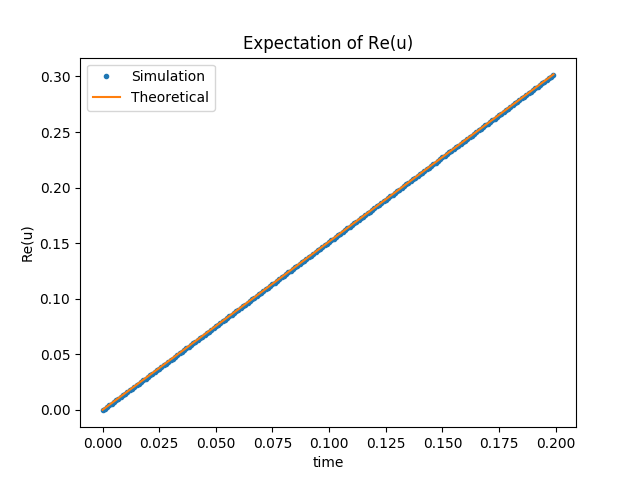
\includegraphics[width = .2\textwidth]{../NumericalSimulation/100k/EuRe.png}
  }\hfill
\subfigure[E(Im(u))]{
  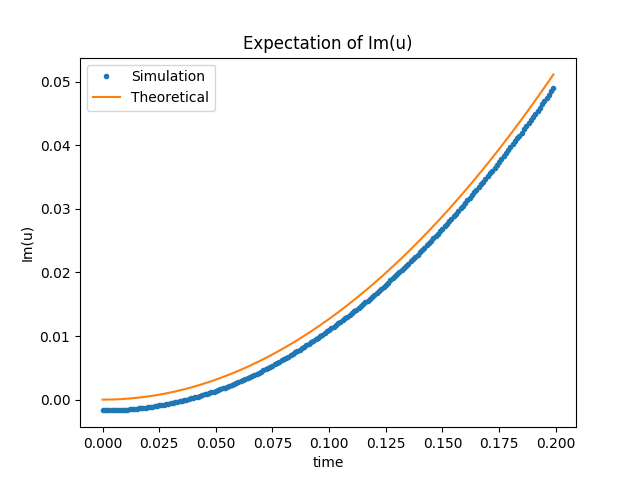
\includegraphics[width = .2\textwidth]{../NumericalSimulation/100k/EuIm.png}
  }\hfill
\subfigure[E(Re(b))]{
  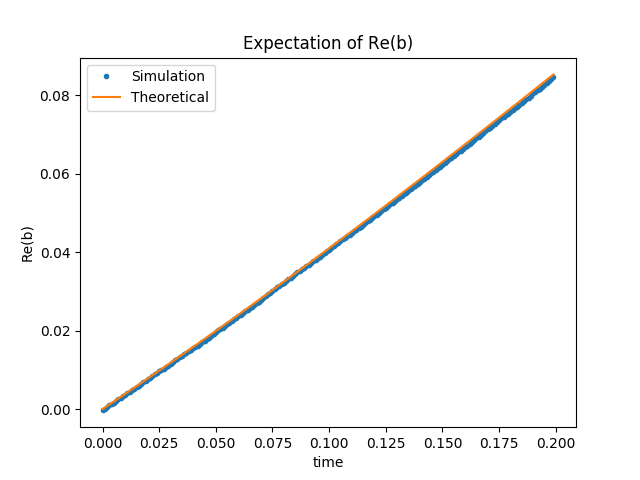
\includegraphics[width = .2\textwidth]{../NumericalSimulation/100k/EbRe.png}
  }\hfill
\subfigure[E(Im(b))]{
  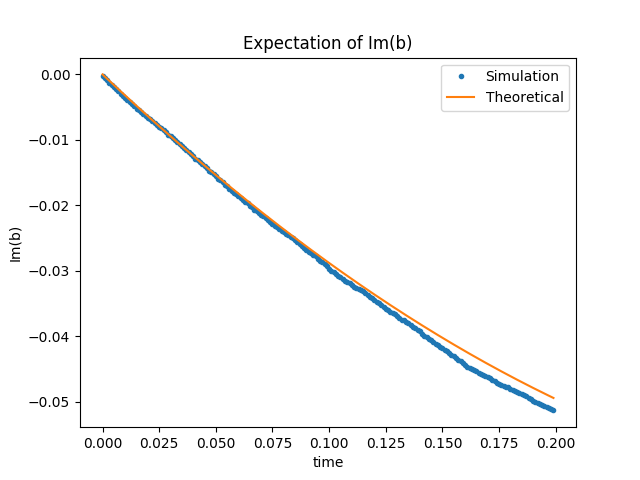
\includegraphics[width = .2\textwidth]{../NumericalSimulation/100k/EbIm.png}
  }\\
\subfigure[E($\gamma$)]{
  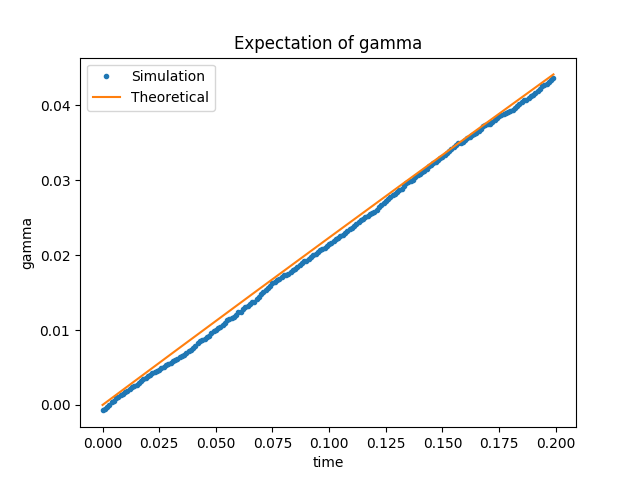
\includegraphics[width = .2\textwidth]{../NumericalSimulation/100k/Egamma.png}
  }\hfill
\subfigure[Var(u)]{
  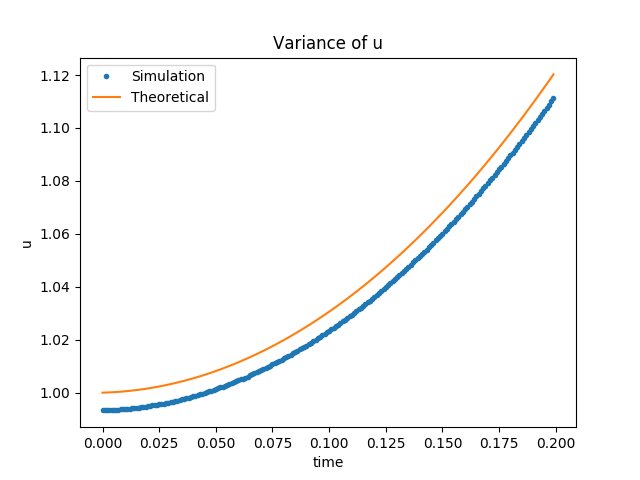
\includegraphics[width = .2\textwidth]{../NumericalSimulation/100k/Varu.png}
  }\hfill
\subfigure[Var(b)]{
  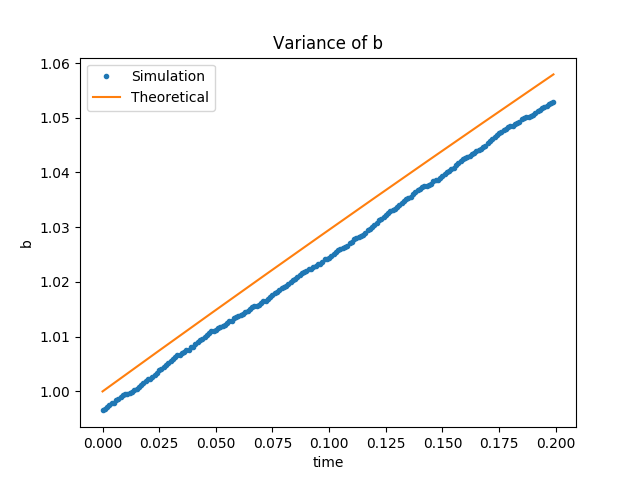
\includegraphics[width = .2\textwidth]{../NumericalSimulation/100k/Varb.png}
  }\hfill
\subfigure[Var($\gamma$)]{
  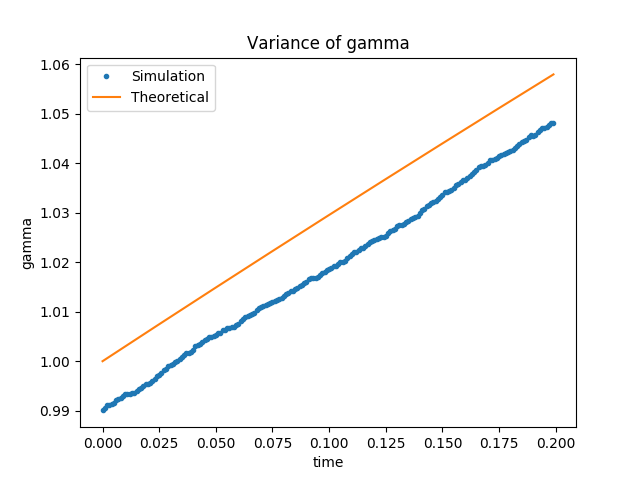
\includegraphics[width = .2\textwidth]{../NumericalSimulation/100k/Vargamma.png}
  }
\caption{Simulation of Expectations and Variances, $n = 10^6$}
\label{Simulation of Expectations and Variances 1}
\end{figure}
}

\frame{\frametitle{Result}
\begin{figure}[!ht]
\centering
\subfigure[$\text{Re}(\Cov(u, u^*))$]{
  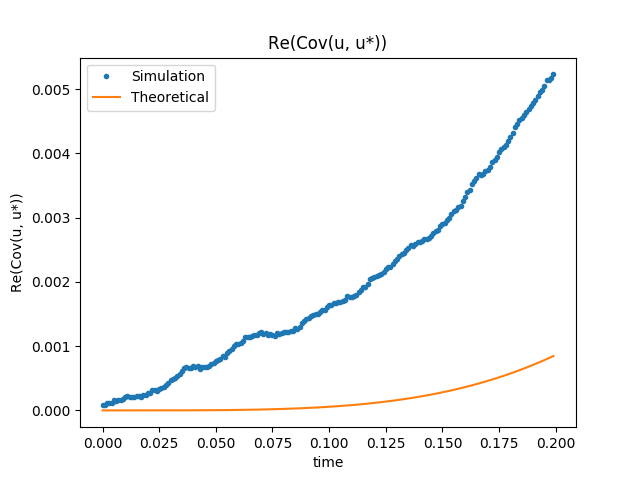
\includegraphics[width = .2\textwidth]{../NumericalSimulation/100k/CovuustarRe.png}
}\hfill
\subfigure[$\text{Im}(\Cov(u, u^*))$]{
  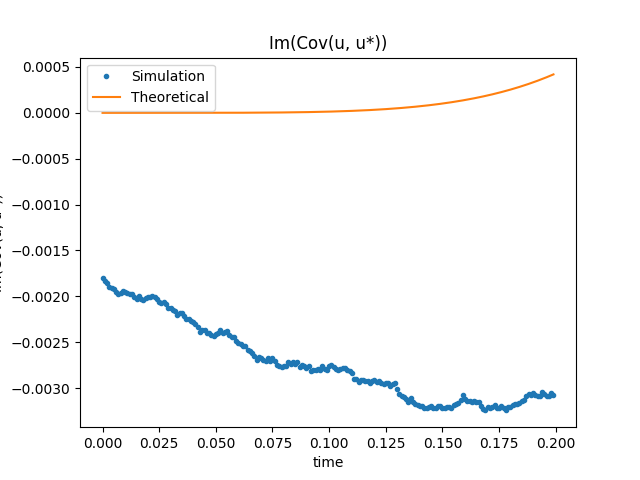
\includegraphics[width = .2\textwidth]{../NumericalSimulation/100k/CovuustarIm.png}
}\hfill
\subfigure[$\text{Re}(\Cov(u, \gamma))$]{
  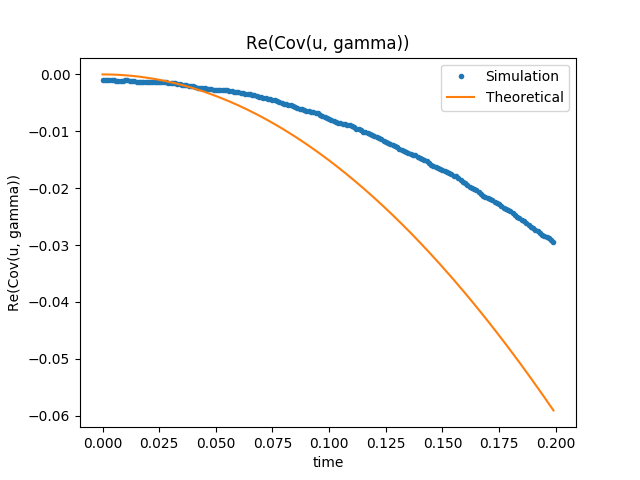
\includegraphics[width = .2\textwidth]{../NumericalSimulation/100k/CovugammaRe.png}
}\hfill
\subfigure[$\text{Im}(\Cov(u, \gamma))$]{
  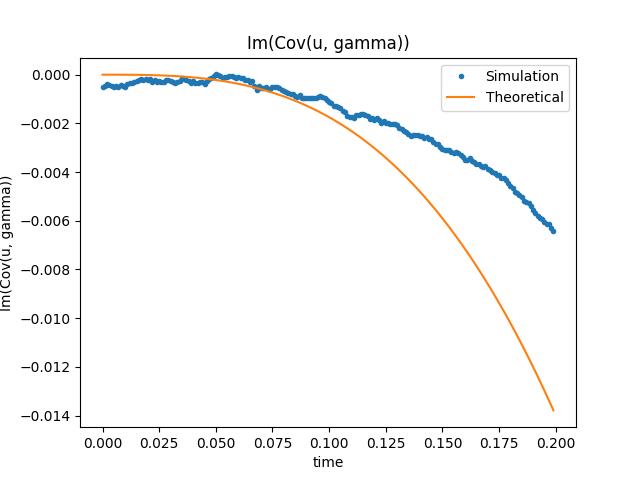
\includegraphics[width = .2\textwidth]{../NumericalSimulation/100k/CovugammaIm.png}
}\\
\subfigure[$\text{Re}(\Cov(u, b))$]{
  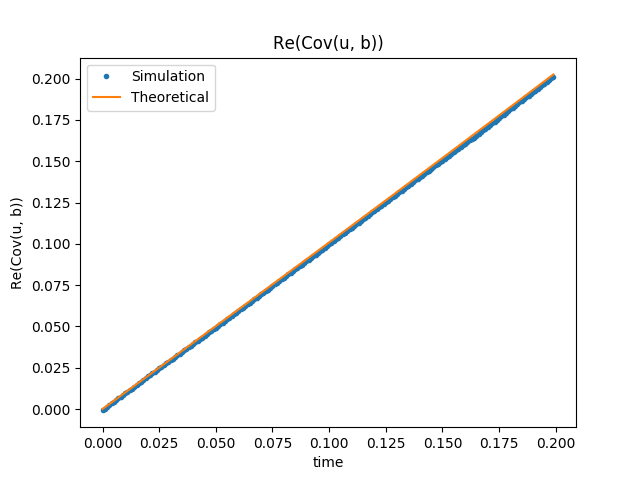
\includegraphics[width = .2\textwidth]{../NumericalSimulation/100k/CovubRe.png}
}\hfill
\subfigure[$\text{Im}(\Cov(u, b))$]{
  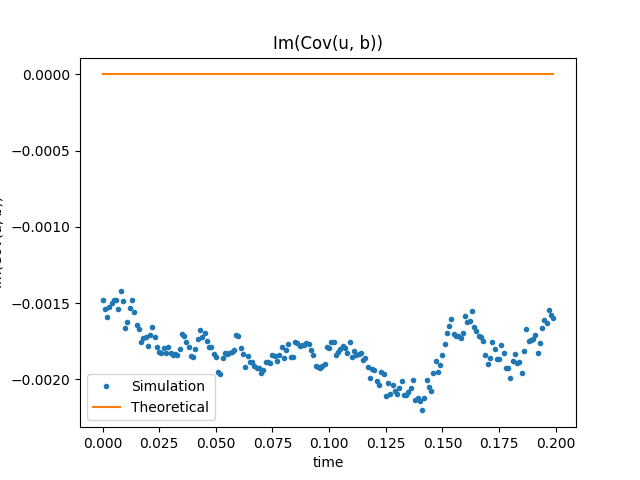
\includegraphics[width = .2\textwidth]{../NumericalSimulation/100k/CovubIm.png}
}\hfill
\subfigure[$\text{Re}(\Cov(u, b^*))$]{
  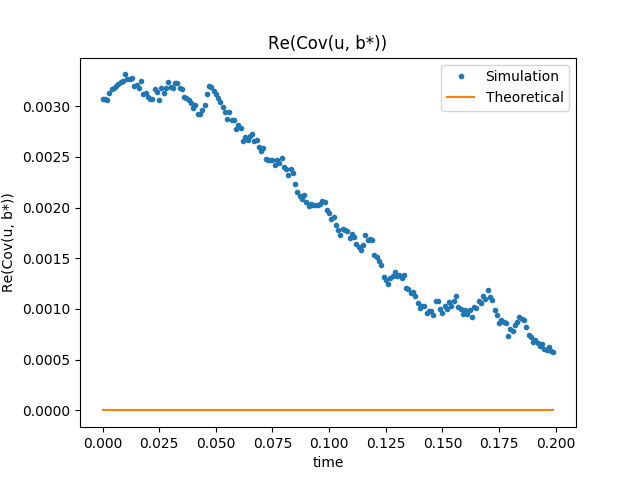
\includegraphics[width = .2\textwidth]{../NumericalSimulation/100k/CovubstarRe.png}
}\hfill
\subfigure[$\text{Im}(\Cov(u, b^*))$]{
  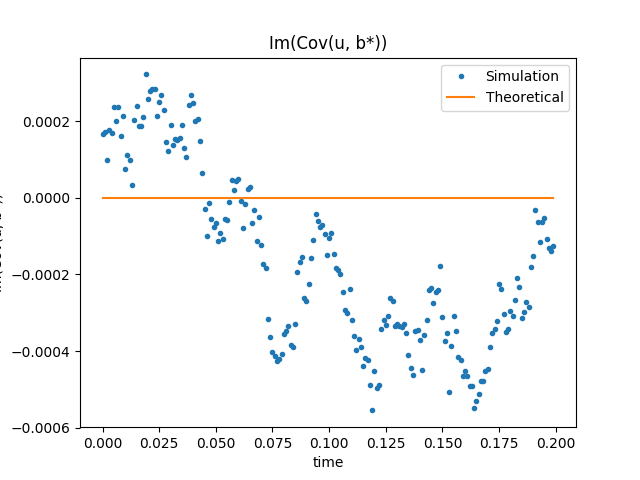
\includegraphics[width = .2\textwidth]{../NumericalSimulation/100k/CovubstarIm.png}
}
\caption{Simulation of Covariances, $n = 10^6$}
\label{Simulation of Covariances 1}
\end{figure}
}

\frame{\frametitle{Results}
\quad Simulate $10^7$ times with $R = 1$, the results are as follows:
\begin{figure}[!ht]
\centering
\subfigure[\text{E}(Re(u))]{
  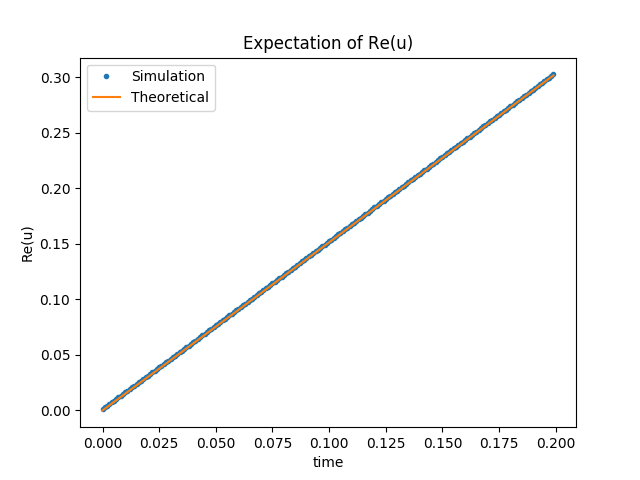
\includegraphics[width = .2\textwidth]{../NumericalSimulation/1m/EuRe.png}
  }\hfill
\subfigure[E(Im(u))]{
  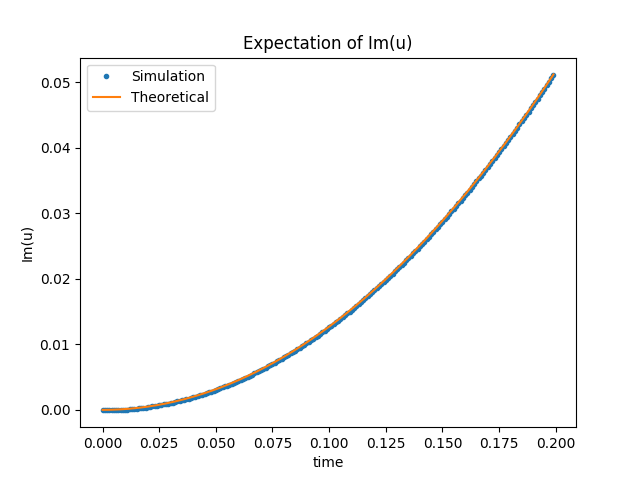
\includegraphics[width = .2\textwidth]{../NumericalSimulation/1m/EuIm.png}
  }\hfill
\subfigure[E(Re(b))]{
  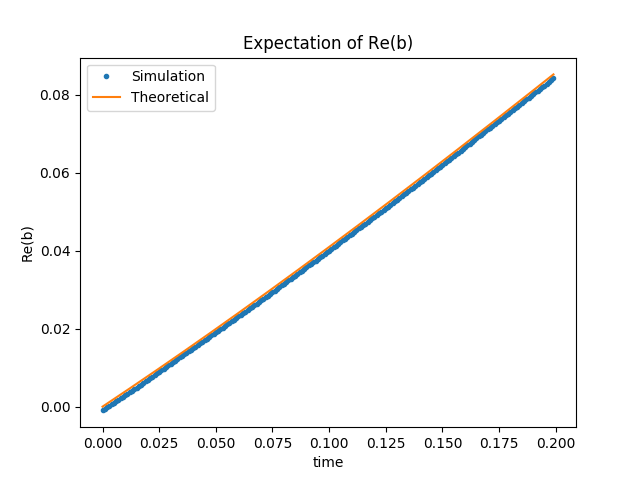
\includegraphics[width = .2\textwidth]{../NumericalSimulation/1m/EbRe.png}
  }\hfill
\subfigure[E(Im(b))]{
  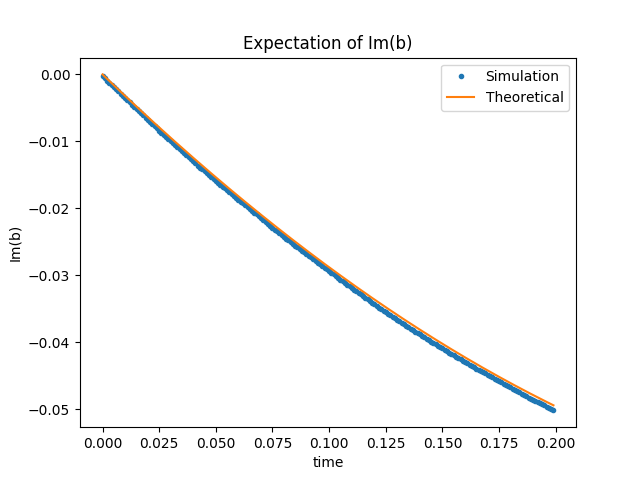
\includegraphics[width = .2\textwidth]{../NumericalSimulation/1m/EbIm.png}
  }\\
\subfigure[E($\gamma$)]{
  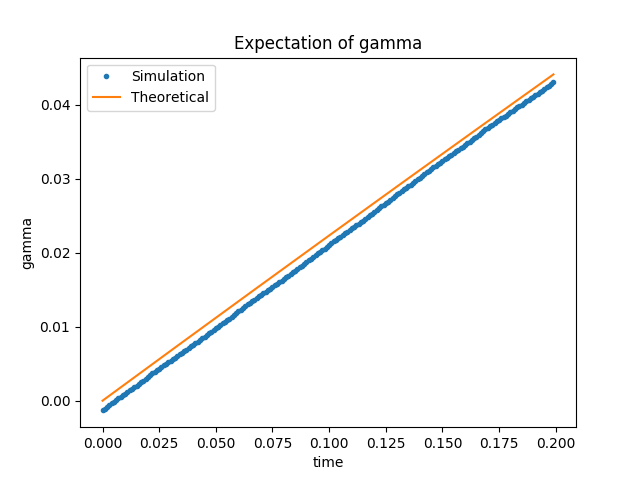
\includegraphics[width = .2\textwidth]{../NumericalSimulation/1m/Egamma.png}
  }\hfill
\subfigure[Var(u)]{
  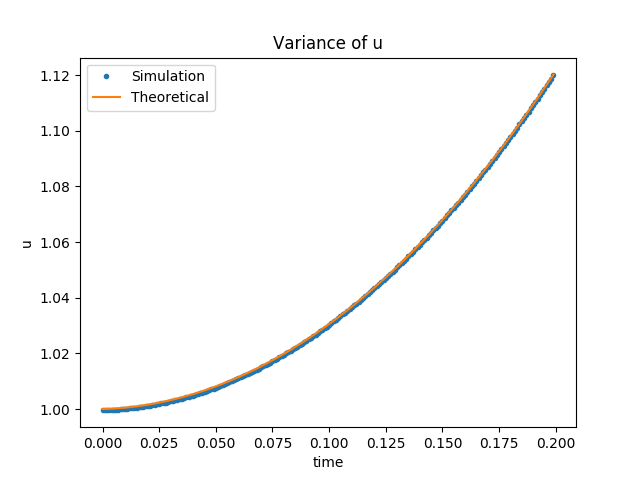
\includegraphics[width = .2\textwidth]{../NumericalSimulation/1m/Varu.png}
  }\hfill
\subfigure[Var(b)]{
  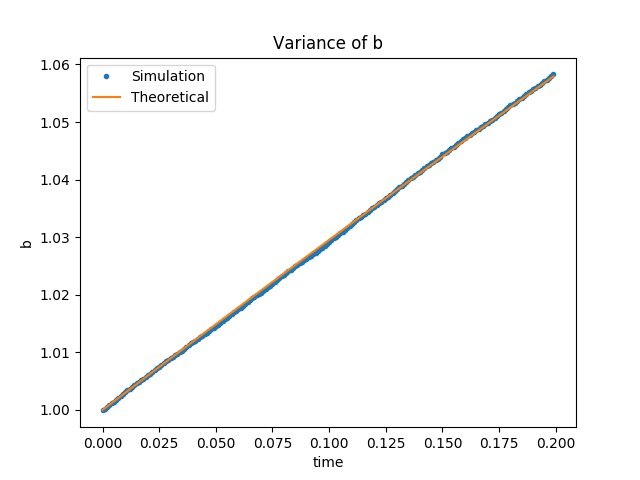
\includegraphics[width = .2\textwidth]{../NumericalSimulation/1m/Varb.png}
  }\hfill
\subfigure[Var($\gamma$)]{
  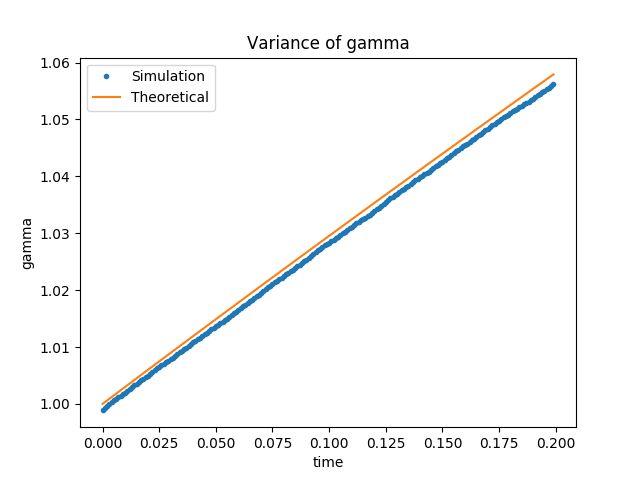
\includegraphics[width = .2\textwidth]{../NumericalSimulation/1m/Vargamma.png}
  }
\caption{Simulation of Expectations and Variances, $n = 10^7$}
\label{Simulation of Expectations and Variances 2}
\end{figure}
}


\frame{\frametitle{Result}
\begin{figure}[!ht]
\centering
\subfigure[$\text{Re}(\Cov(u, u^*))$]{
  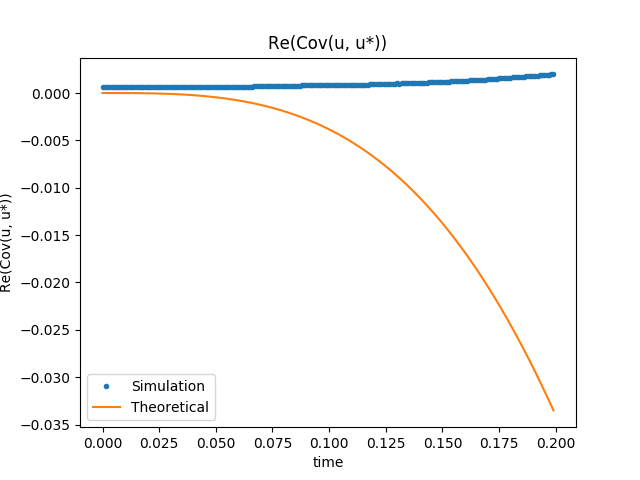
\includegraphics[width = .2\textwidth]{../NumericalSimulation/1m/CovuustarRe.png}
}\hfill
\subfigure[$\text{Im}(\Cov(u, u^*))$]{
  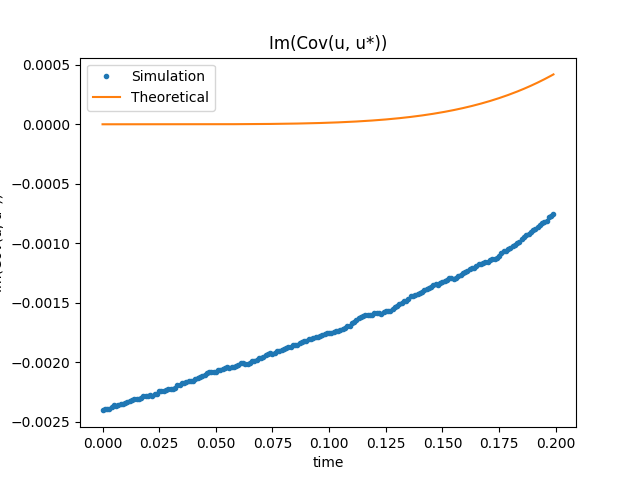
\includegraphics[width = .2\textwidth]{../NumericalSimulation/1m/CovuustarIm.png}
}\hfill
\subfigure[$\text{Re}(\Cov(u, \gamma))$]{
  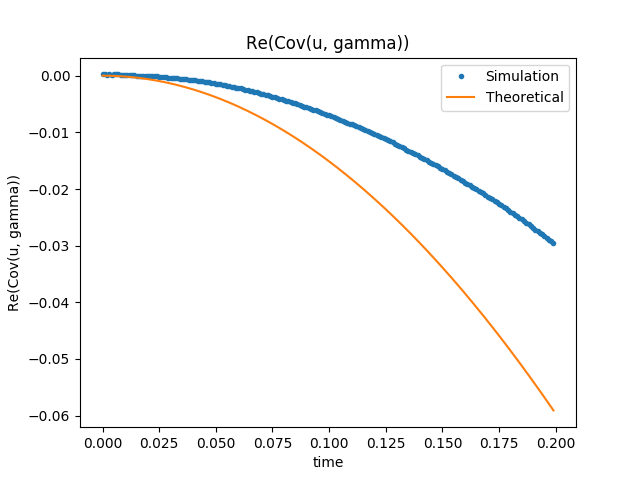
\includegraphics[width = .2\textwidth]{../NumericalSimulation/1m/CovugammaRe.png}
}\hfill
\subfigure[$\text{Im}(\Cov(u, \gamma))$]{
  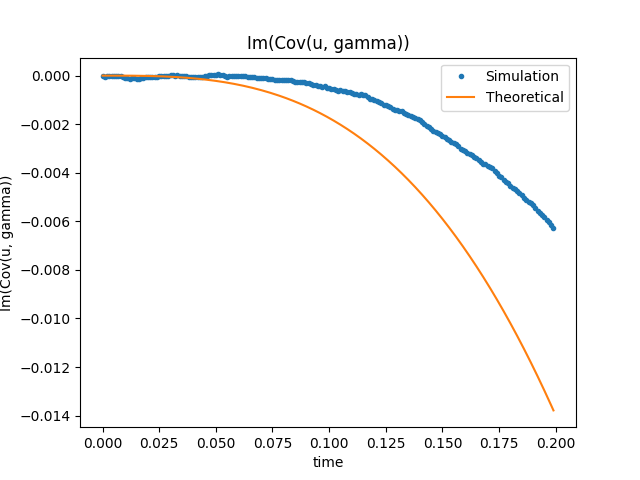
\includegraphics[width = .2\textwidth]{../NumericalSimulation/1m/CovugammaIm.png}
}\\
\subfigure[$\text{Re}(\Cov(u, b))$]{
  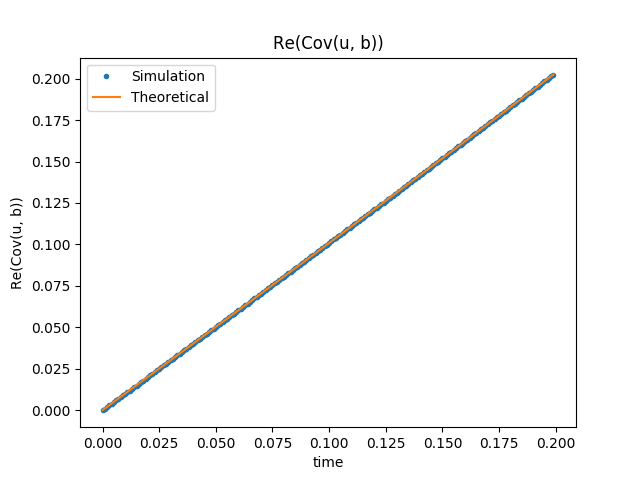
\includegraphics[width = .2\textwidth]{../NumericalSimulation/1m/CovubRe.png}
}\hfill
\subfigure[$\text{Im}(\Cov(u, b))$]{
  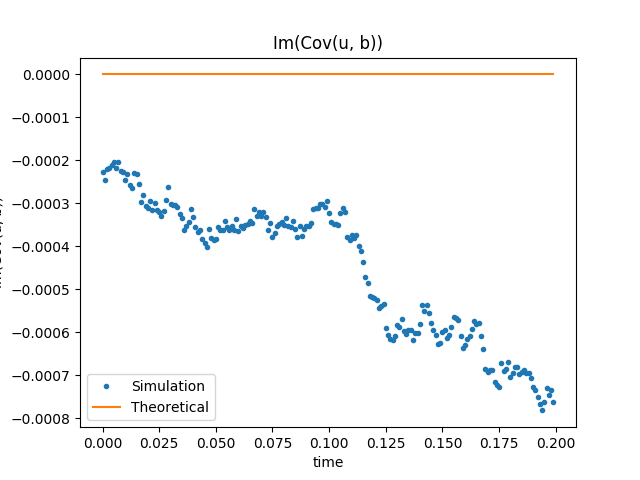
\includegraphics[width = .2\textwidth]{../NumericalSimulation/1m/CovubIm.png}
}\hfill
\subfigure[$\text{Re}(\Cov(u, b^*))$]{
  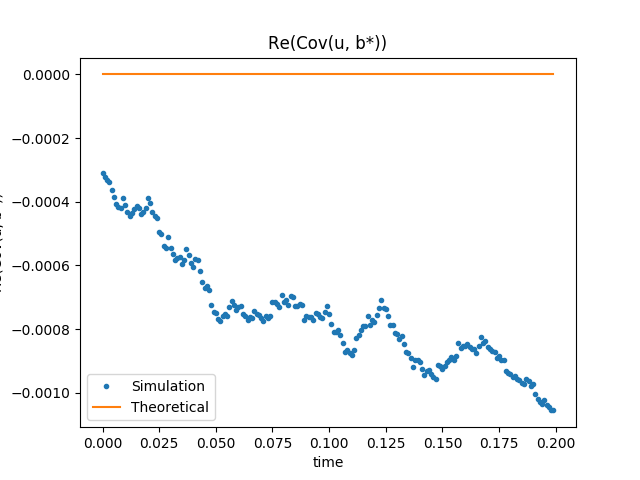
\includegraphics[width = .2\textwidth]{../NumericalSimulation/1m/CovubstarRe.png}
}\hfill
\subfigure[$\text{Im}(\Cov(u, b^*))$]{
  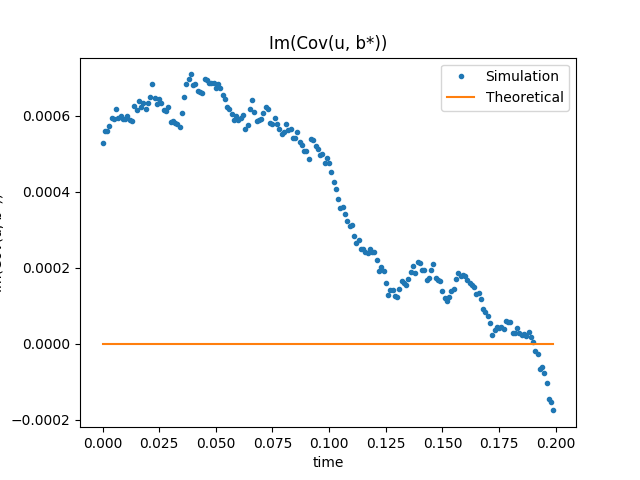
\includegraphics[width = .2\textwidth]{../NumericalSimulation/1m/CovubstarIm.png}
}
\caption{Simulation of Covariances, $n = 10^7$}
\label{Simulation of Covariances 2}
\end{figure}
}

\frame{\frametitle{Discussion}
From the simulation results we find that the simulation of expectations fit the theoretical results satisfyingly. 

For the results of Variances and Covariances, \\[5pt]
\begin{itemize}
\item When $n = 10^6$, the error of variances is about $O(10^{-2})\sim O(10^{-3})$, error of covariances is about $O(10^{-2})\sim O(10^{-3})$. \\[10pt]
\item When $n = 10^7$, the error of $\Var(u), ~\Var(b)$ is about $O(10^{-5})$, and error of $\Var(\gamma)$ is about $O(10^{-3})\sim O(10^{-4})$, error of $\Cov(u, u^*), ~\Cov(u, \gamma)$ is about $O(10^{-3})$, error of $\Cov(u, b), ~\Cov(u, b^*)$ is $O(10^{-4})$.
\end{itemize}
}
\frame{\frametitle{Discussion}
One can find the simulation errors decrease with the growth of simulations. Thus one could believe that when $n\to\infty$, the simulation would converge to the theoretical result. In fact, error of simulation comes from that initial values are all random variables; according to Law of large numbers, the errors would converge to 0 when $n\to\infty$.\\[10pt]

We can get third-order and fourth-order statistics of $u, b, \gamma$ with the same methods, which could be written in a form of multiple integrals of statistics of initial values.
}

% \begin{frame}{References}
%     \bibliographystyle{amsalpha}
%     \bibliography{../../../CONFIG/Latex-bib/Chuan}
% \end{frame}

\frame{
	\quad\quad\centering{ \Huge Thank you!}
}
\end{document}
